\documentclass{beamer}
\usepackage{xgreek}
\usepackage{xltxtra}
\usepackage{graphicx}
\useoutertheme{shadow}
\usetheme{Singapore}
\setsansfont[Mapping=tex-text]{GFS Didot}
\setmonofont[Mapping=tex-text]{DejaVu Sans Mono}
%Remove navigation symbols
\setbeamertemplate{navigation symbols}{}
%effect so overlays not yet revealed will faintly appear
\setbeamercovered{dynamic}

\title[ScorpioFS]{ScorpioFS\\Κατανεμημένο ομότιμο σύστημα αρχείων}
\author{Αντώνης Κουζούπης}
\institute{Πανεπιστήμιο Πειραιώς\\Τμήμα Πληροφορικής}
\date{\today}
\logo{
\includegraphics[scale=0.5]{images/unipi_logo.jpg}}

\begin{document}
\frame{
    \titlepage
}
\section{Εισαγωγή}
\subsection{}
\frame{
\frametitle{Τι είναι το ScorpioFS}
\begin{itemize}
\item Σύστημα αποθήκευσης αντιγράφων ασφαλείας \\ \footnotesize 
Παρέχει στο χρήστη ένα τοπικά προσαρτημένο σύστημα αρχείων το οποίο αποθηκεύει
τα περιεχόμενά του στο δίκτυο.\normalsize
\pause
\item Δίκτυο ομότιμα συνδεδεμένων υπολογιστών \\
\footnotesize Αποτελεί ένα δίκτυο υπολογιστών που παρέχουν
στην υπηρεσία μία τοπική αποθήκη καθώς και μία λειτουργία αντιγραφής των αρχείων
μεταξύ των κόμβων για την εξασφάλιση της διαθεσιμότητας των δεδομένων. Όλοι οι κόμβοι 
στο δίκτυο είναι ομότιμα συνδεδεμένοι (peer--to--peer).\normalsize
\pause
\item Κατανεμημένο σύστημα \\
\footnotesize Το σύστημα αποθήκευσης αρχείων είναι πλήρως αποκεντρωμένο. Όλοι οι
κόμβοι στο δίκτυο έχουν ισότιμα δικαιώματα. Κληρονομεί τα πλεονεκτήματα και τα
μειονεκτήματα των κατανεμημένων συστημάτων.\normalsize
\end{itemize}
}
\subsection{}
\frame{
\frametitle{Τα μέρη του ScorpioFS \\ (Chord)(Σκατά Τίτλος!!!)}
Το μέρος του \emph{ScorpioFS} που υλοποιεί το
Chord πρωτόκολλο. Είναι υπεύθυνο για την εύρεση των κόμβων που είναι
αποθηκευμένα τα δεδομένα, την εισαγωγή και τη διαγραφή ενός κόμβου από το δίκτυο
και για την αντιγραφή των αρχείων. Γενικά είναι υπεύθυνο για το δικτυακό
κομμάτι.
}

\frame{
\frametitle{Τα μέρη του ScorpioFS \\ (Fuse)(Σκατά Τίτλος!!!)}
Υλοποιεί το τοπικό σύστημα αρχείων που αντιλαμβάνεται ο
χρήστης. Υλοποιεί τις περισσότερες λειτουργίες ενός συστήματος αρχείων όπως
δημιουργία, διαγραφή, επεξεργασία, αντιγραφή κτλ. Χωρίζει μεγάλα αρχεία σε
μικρότερα του 1MB και επικοινωνεί με το \textbf{Chord} κομμάτι για την αποστολή
και αποδοχή δεδομένων.
}

\frame{
\frametitle{Τα μέρη του ScorpioFS \\ (Console)(Σκατά Τίτλος!!!)}
Κονσόλα διαχείρισης των κόμβων του δικτύου. Εκτελεί διάφορες λειτουργίες μαζικά
στους κόμβους όπως δημιουργία ή καταστροφή, περισυλλογή των στατιστικών.
Λειτουργεί ανεξάρτητα από το \textbf{Chord} και \textbf{Fuse} κομμάτι και
επιτελεί επικουρικό ρόλο στο σύστημα.
}

\subsection{}
\frame{
\frametitle{Σχεδιάγραμμα Δικτύου}
\begin{figure}
    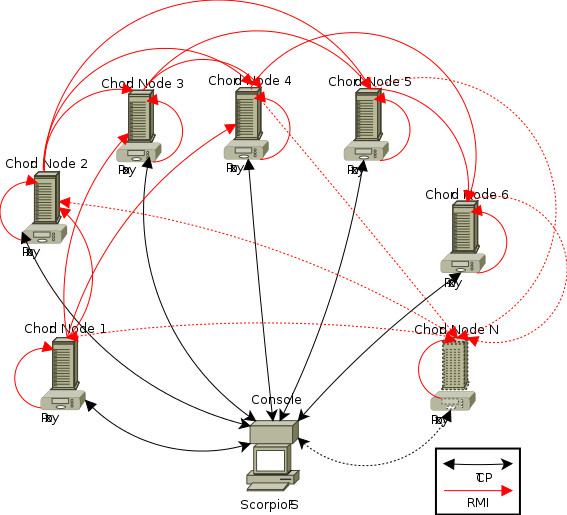
\includegraphics[scale=0.4]{images/scorpio_console.png}
\end{figure}
}

\section{Chord}

\subsection{}
\frame{
\transboxin
\frametitle{Το πρωτόκολλο Chord}
\begin{itemize}
    \item University of California, Berkeley \& MIT Laboratory for Computer
Science -- SIGCOMM'01
    \item Επεκτάσιμο πρωτόκολλο για αναζήτηση σε ένα δυναμικό peer--to--peer
σύστημα με συχνές αφίξεις και αναχωρήσεις κόμβων.
    \item Αποθηκεύει ζευγάρια key/data στον κατάλληλο κόμβο.
    \item Δοθέντος ενός κλειδιού το αντιστοιχίζει σε ένα κόμβο.
    \item \emph{Consistent hashing} για εξισορρόπηση του φόρτου εργασίας, κάθε κόμβος
είναι υπεύθυνος για περίπου τον ίδιο αριθμό κλειδιών, ελάχιστες μετακινήσεις
κλειδιών όταν ένας κόμβος μπαίνει ή βγαίνει από το σύστημα.
\end{itemize}
}

\frame{
\frametitle{Το πρωτόκολλο Chord}
\begin{itemize}
    \item Σε ένα σύστημα με N κόμβους, κάθε κόμβος κρατάει πληροφορία για μόνο
$\bigcirc{(\log{N})}$ άλλους κόμβους.
    \item Επιλύει όλες τις αναζητήσεις μέσω $\bigcirc{(\log{N})}$ μηνυμάτων προς
άλλους κόμβους.
    \item Το πρωτόκολλο παρέχει μία $lookup(key)$ συνάρτηση που βρίσκει την IP
διεύθυνση του κόμβου που είναι υπεύθυνος για το κλειδί.
    \item Το Chord ενημερώνει τους κόμβους για τις αλλαγές των κλειδιών που
είναι υπεύθυνοι.
    \item Όταν ο N-οστός κόμβος έρθει ή φύγει από το σύστημα μόνο
$\bigcirc{(\frac{1}{N})}$ κλειδιά μετακινούνται.
\end{itemize}
}

\subsection{}
\frame{
\frametitle{Χαρακτηριστικά του Chord}
\begin{itemize}
    \item \textbf{Load balance} -- Το Chord λειτουργεί σαν κατανεμημένη
συνάρτηση κατακερματισμού διαμοιράζοντας τα κλειδιά σε όλους τους κόμβους.
    \item \textbf{Decentralization} -- Κανένας κόμβος δεν είναι πιο σημαντικός
από τους άλλους. Κατάλληλο για χαλαρά συνδεδεμένες peer--to--peer εφαρμογές.
    \item \textbf{Scalability} -- Το κόστος μιας αναζήτησης αυξάνεται
λογαριθμικά σε σχέση με το πλήθος των κόμβων.
    \item \textbf{Availability} -- Ρυθμίζει αυτόματα το δίκτυο ώστε να
``κρύψει'' από την εφαρμογή τις αποχωρήσεις και τις αφίξεις νέων κόμβων.
    \item \textbf{Flexible naming} -- Δεν θέτει κάποιο περιορισμό στη μορφή των
κλειδιών.
\end{itemize}
}

\frame{
\frametitle{Consistent Hashing}
Ένα κλειδί $\kappa$ ανατίθεται στο πρώτο κόμβο που το αναγνωριστικό του ισούται
ή ακολουθεί το $\kappa$. Ο κόμβος αυτός ονομάζεται $successor$ κόμβος του
κλειδιού $\kappa$.

\begin{figure}
    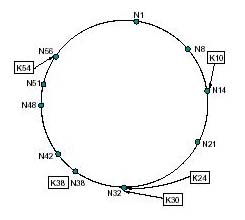
\includegraphics[scale=2]{images/chord_hashing.jpg}
\end{figure}
}

\subsection{}
\frame{
\frametitle{Finger Table}
Κάθε κόμβος $n$ κρατάει ένα πίνακα δρομολόγησης με $m (\bigcirc{(log{N})})$
εγγραφές που ονομάζεται \emph{finger table}. Το i-οστό στοιχείο του πίνακα
περιέχει το αναγνωριστικό του πρώτου κόμβου που επιτυγχάνει τον $n$ κατά
λιγότερο $2^{i-1}$.

\begin{figure}
    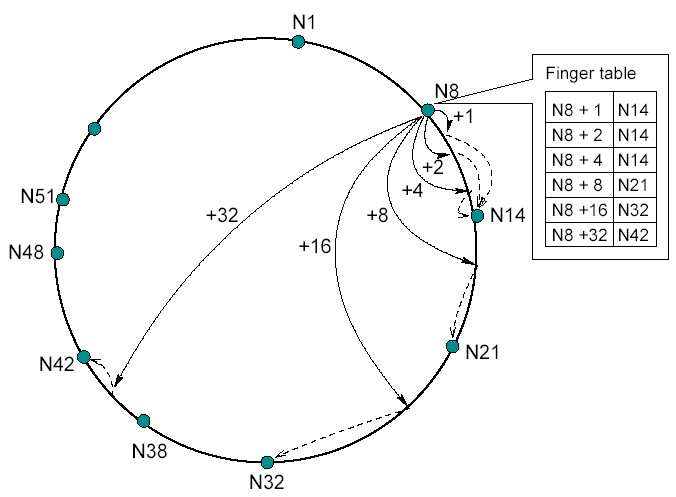
\includegraphics[scale=0.3]{images/chord_finger.png}
\end{figure}
}

\frame{
\frametitle{Finger Table}
Το πρώτο στοιχείο στον πίνακα του κόμβου $8$ είναι ο κόμβος $14$ αφού είναι ο πρώτος
κόμβος που έπεται το $(8+2^0)\mod{2^6}=9$. Αντίστοιχα, το τελευταίο στοιχείο του
πίνακα είναι ο κόμβος $42$, καθώς είναι ο πρώτος κόμβος που έπεται του
$(8+2^5)\mod{2^6}=40$.
}

\frame{
\frametitle{Finger Table}
\begin{itemize}
    \item Κάθε κόμβος κρατάει πληροφορία για ένα μικρό αριθμό κόμβων. Επίσης αυτοί
οι κόμβοι είναι οι πιο κοντινοί του.
    \item Γενικά το finger table ενός κόμβου δεν περιέχει αρκετή πληροφορία ώστε να
καθορίσει τον successor ενός τυχαίου κλειδιού $k$.
    \item Η διαδικασία για την εύρεση ενός successor μπορεί να γίνει αναδρομικά
και στους κόμβους του finger table ενός κόμβου $n$, εάν το κλειδί προς αναζήτηση
είναι πιο μακρυά από τον τελευταίο κόμβο στο finger table του κόμβου $n$.
    \item Καθώς κάθε κόμβος έχει εγγραφές σε διαστήματα της δύναμης του δύο, μπορεί
να προωθήσει μία ερώτηση τουλάχιστον στο μισό δρόμο.
\end{itemize}
}

\frame{
\frametitle{Finger Table}
Εάν υποθέσουμε ότι ο κόμβος $8$ θέλει να βρει τον successor για το κλειδί $54$.
Αφού η μεγαλύτερη εγγραφή στο finger table του κόμβου $8$ που προηγείται του $54$
είναι ο κόμβος $42$, ο κόμβος $8$ θα ρωτήσει τον κόμβο $42$ να εξυπηρετήσει την
ερώτηση.

Ο κόμβος $42$ βρίσκει ότι η μεγαλύτερη εγγραφή που προηγείται του $54$ είναι ο
κόμβος $51$. Ο κόμβος $51$ θα βρει ότι ο successor του $54$ είναι ο
κόμβος $56$. Τελικά ο κόμβος $51$ θα επιστρέψει στον κόμβο $8$ ότι ο successor
του κλειδιού $54$ είναι ο κόμβος $56$.
}

\subsection{}
\frame{
\frametitle{Εισαγωγή Κόμβου}
Ένας νέος κόμβος $n$ εισέρχεται στο σύστημα:
\begin{enumerate}
    \item Ο κόμβος $n$ καλεί όποιο κόμβο γνωρίζει και του ζητάει να του βρει τον
successor του.
    \item Ο κόμβος $n$ αντιγράφει όσα στοιχεία από το finger table του successor
του είναι μικρότερα από $n$.
    \item Ανά τακτά διαστήματα γίνεται ``stabilize'' στο δίκτυο. Ο τρέχοντας
κόμβος ρωτάει τον successor του, για τον predecessor του successor του. Με αυτό
τον τρόπο ένας νέος κόμβος γίνεται γνωστός στο δίκτυο.
    \item Κάθε κόμβος ελέγχει περιοδικά τον predecessor του για ενημερώσει τυχών
λανθασμένες εγγραφές.
\end{enumerate}
}

\frame{
\frametitle{Εισαγωγή Κόμβου}
Ο κόμβος $26$ εισέρχεται στο σύστημα μεταξύ των κόμβων $21$ και $32$. Ο κόμβος
$26$ βρίσκει τον successor του (κόμβος $32$). Ο κόμβος $26$ αντιγράφει όλα τα
κλειδιά του successor του που είναι μικρότερα από $26$. Με τη διαδικασία του
``stabilize'' ενημερώνεται ο κόμβος $21$, ότι ο successor του είναι ο κόμβος $26$

Να scan-aro και να βάλω το παράδειγμα από το paper.
}

\subsection{}
\frame{
\frametitle{Αποχώρηση Κόμβου}
Για να αυξηθεί η διαθεσιμότητα του συστήματος, κάθε κόμβος κρατάει μία λίστα από
successors ($\Omega(\log{N})$) και όχι μόνο έναν. Εάν μία κλήση προς ένα successor αποτύχει, τότε
γίνεται κλήση στον αμέσως επόμενο. Θα πρέπει να αποτύχουν όλοι οι κόμβοι για να
υπάρχει δυσλειτουργία.\\[1em]

Ένας κακόβουλος χρήστης θα μπορούσε κάνει ορισμένους κόμβους να αποτύχουν αλλά
όχι συγκεκριμένους κατ' επιλογή κόμβους.
}

\frame{
\frametitle{Αποχώρηση Κόμβου}
Η εφαρμογή που χρησιμοποιεί το Chord πρωτόκολλο, ScorpioFS, αντιγράφει τα
δεδομένα και σε άλλους κόμβους. Έτσι για τα ίδια δεδομένα είναι υπεύθυνοι
παραπάνω από ένας κόμβοι αλλά με άλλο κλειδί.\\[1em]

Μία οικειοθελής αποχώρηση μπορεί να χειριστεί σαν μία αποτυχία του κόμβου.
}
\section{FUSE}
\section{ScorpioFS}
\section{Πειράματα}
\section{Εκτέλεση}
\section{Επίδειξη}
\section{Μελλοντική Εργασία}
\end{document}
